\documentclass[a4paper,10pt]{article}
%\usepackage[latin1]{inputenc} % Paquetes de idioma
\usepackage[utf8]{inputenc} % Paquetes de idioma (Este encoding toma acentos :) )
\usepackage[spanish]{babel} % Paquetes de idioma
\usepackage{graphicx} % Paquete para ingresar gráficos
\usepackage{grffile}
\usepackage{hyperref}
\usepackage{fancybox}
\usepackage{amsmath}
\usepackage{amsfonts}
\usepackage{listings}
\usepackage{float}
% Paquetes de macros de Circuitos
%\usepackage{pstricks}
\usepackage{tikz}

% Encabezado y Pié de página
\usepackage{fancyhdr} % Paquete para encabezados y pie de página
\pagestyle{fancy} % Sin esta línea no se imprimiría el encabezado en todas las páginas

\fancyhf{} %  Borra el encabezado anterior (Por defecto escribe el títutlo de la sección en la que se encuentra la hoja
\setlength{\headheight}{22.55pt}
\fancyhead[L]{
	{\textsf{Facultad de Ingenier\'ia $-$ Universidad de Buenos Aires \\ 66.44 Instrumentos Electrónicos}}
}
%\addtocounter{page}{5}
\fancyhead[R]{\thepage}

\renewcommand{\footrulewidth}{0.4pt} % Ajusta el tamaño de las líneas separadoras en el pié de página
\renewcommand{\headrulewidth}{0.4pt} % Ajusta el tamaño de las líneas separadoras en el encabezado

\fancyfoot[L]{
	{\textsf{Trabajo Pr\'actico N$^{\circ}4$}: Mediciones de impedancias} \\
	{\textsf{Integrantes: Eduardo Sanchez, Francisco Soler}}
	}
		

% Carátula del Trabajo
\title{ \author{} % Lo pongo para que el warning no moleste :p
\setlength{\unitlength}{1cm} %  Especifica la unidad de trabajo
\thispagestyle{empty}

\begin{picture}(18,0)
\put(0,0){
\includegraphics[width=1.5cm, height=3cm]{Logo1.png}}

\put(10.5,0){
\includegraphics[width=3cm, height=3cm]{Logo2.png}}

\end{picture}
\\[1.5cm]
\begin{center}
	\textbf{{\Huge Facultad de Ingenier\'ia \\ Universidad de Buenos Aires}}\\[2cm]
	{66.44 Instrumentos Electrónicos}\\[0.5cm]
	{Trabajo Pr\'actico N$^{\circ}3$: Mediciones de impedancias}\\[2.5cm]
\end{center}

\begin{flushleft}
	\textbf{Integrantes:} \\[1cm]

	\begin{tabular}{|c|c|c|}
		\hline
		\textbf{\normalsize Padr\'on} & \textbf{\normalsize Nombre} & \textbf{\normalsize Email} \\
		\hline
		\normalsize 92903 & \normalsize Sanchez, Eduardo Hugo & \normalsize hugo\_044@hotmail.com \\
		\hline
		\normalsize 91227 & \normalsize Soler, Jos\'e Francisco & \normalsize francisco.\_tw@hotmail.com \\
		\hline
		\normalsize xxx & \normalsize Wawrynczak, Claudio  & \normalsize claudiozak@gmail.com \\
		\hline
	\end{tabular}
\end{flushleft}
\date{} % Hace que no se imprima la fecha en la cual se compilo el .tex
 }

\begin{document}
	\maketitle % Hace que el título anterior sea el principal del documento
	\newpage

	\tableofcontents % Esta línea genera un indice a partir de las secciones y 
					 % subsecciones creadas en el documento
	\newpage


	\section{Objetivo}
	
	\indent	El objetivo de este trabajo pr\'actico consiste en conocer el funcionamiento del analizador de espectro y del analizador de redes y mostrar algunos de sus m\'ultiples usos posibles.
	
	\newpage
	\section{Introducci\'on}
	\subsection{Analizador de espectro}
	Un analizador de espectro es b\'asicamente un instrumento que permite visualizar la composici\'on espectral de frecuencias de una se\~nal de entrada. Un diagrama en bloques simplificado puede observarse en la Figura \ref{diagramadebloques}. En la Figura se puede observar que la se\~nal de entrada pasa inicialmente por un atenuador y por un filtro pasabajos (cuyo uso determina sin ambig\"uedad el rango de frecuencias con las que se opera, aunque si se lo elimina permite extender el rango de frecuencias del analizador ). Luego pasa a un multiplicador donde se multiplica con la se\~nal generada por un oscilador local estable. A la salida del multiplicador se encuentran se\~nales cuyas frecuencias son sumas y diferencias de las frecuencias del oscilador local y de la se\~nal de entrada. Las componentes m\'as relevantes se encuentran en $f=f_{osc}-f_{\text{se\~nal}}$ y $f=f_{osc}+f_{\text{se\~nal}}$, pero en general, cuando se utiliza el filtro pasabajo de entrada la componente que interesa es solamente $f=f_{osc}-f_{\text{se\~nal}}$.
	Si alguna de estas se\~nales producidas tiene la frecuencia del filtro pasabanda intermedio, $f_{IF}$, \'esta es luego amplificada logar\'itmicamente (la escala generalmente utilizada en pantalla es en decibeles), rectificada por un detector de envolvente, filtrada por un filtro de video y es utilizada para establecer la se\~nal vertical de la pantalla.
	Con respecto al eje horizontal (el de frecuencias), un generador de rampa controla su barrido de izquierda a derecha. A su vez este mismo generador se encarga de controlar la frecuencia del oscilador local, la cual var\'ia proporcionalmente con la tensi\'on de la rampa. De esta forma se pueden barrer las frecuencias presentes en la se\~nal de entrada y mostrarlas en pantalla.
	\begin{figure}[!htb]
					\centering
					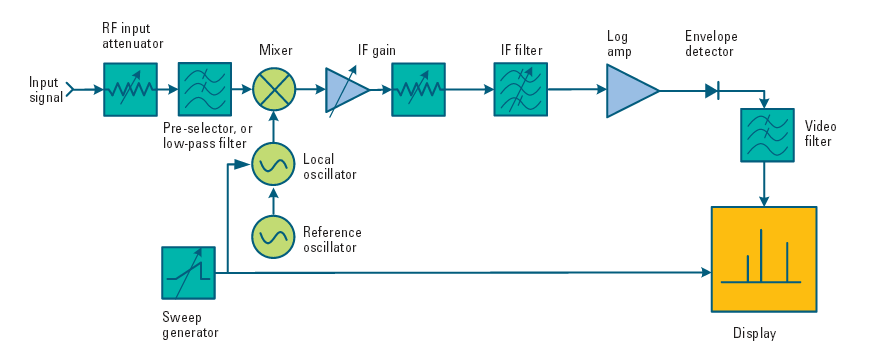
\includegraphics[width=12cm]
					{Imagenes/diagram.PNG}
					\caption{Diagrama en bloques de un analizador de espectro superheterodino}
					\label{diagramadebloques} 
			\end{figure}
	\newpage
	\subsection{Analizador de redes}
	\section{Desarrollo}
	\subsection{Mediciones con el analizador de espectro}
\indent Para llevar a cabo las mediciones, se utilizan los siguientes
		instrumentos:
		\begin{itemize}
			\item Analizador de espectro HM 5006
			\item Analizador de espectro PSA 6000
			\item Generador de funciones Agilent N9310A
			\item Generador de funciones Siglent SDG1050
			\item Cable coaxil para conexi\'on de los instrumentos
		\end{itemize}	
		%HUGO
		\subsubsection{Selectividad}
		La resoluci\'on en frecuencia de un analizador de espectro es su capacidad para poder distinguir 2 se\~nales senoidales de la misma amplitud. Este valor se especifica como el ancho de banda de los filtros FI cuando su respuesta cae $3~dB$. 
		Sin embargo, si las se\~nales es\'an separadas en la frecuencia de resoluci\'on pero con diferente amplitud puede ocurrir que una quede enmascarada dentro de la otra. De esta manera surge otra especificaci\'on que es la selectividad, la cual se define como la relaci\'on entre el ancho de banda cuando la respuesta cae $60~dB$ y cuando cae $3~dB$. Matem\'aticamente 
		$$S=\frac{BW(-60~dB)}{BW(-3~dB)}$$
	
		En esta secci\'on se obtiene la selectividad de los analizadores de espectro HM 5006 y PSA 6000 con diferentes resoluciones. Para ello se conectan por medio de un cable coaxil a un generador Agilent N9310A que produce un se\~nal senoidal de $100~MHz$. En la Tabla \ref{selectividad} se puede observar los resultados obtenidos. En la Figura \ref{Selec} se pueden observar los espectros obtenidos por el analizador PSA 6000, utilizando resoluciones diferentes.
		La incerteza relativa de la frecuencia en el analizador HM 5006 es del $10\%$, mientras que la  del analizador PSA 6000 sigue la siguente f\'ormula
		$$\Delta f=\pm\left(f\cdot \%_{ref} +3\%\cdot Span+50\%\cdot RBW \right)$$
		%Cual es el \%_{ref}, el manual lo nombra una sola vez jajaja pero no dice que valor tiene.
		
		\begin{table}[!htp]
			\centering
			\begin{tabular}{|c|c|c|c|c|}
				\hline
				Analizador & Resoluci\'on & $BW(-60~dB)$ & $BW(-3~dB)$ & Selectividad \\
				\hline
				HM 5006 & $250~kHz$& $300~kHz~\pm~30~kHz$ & 
				$900~kHz~\pm~90~kHz\%$ &$ 3~\pm~0.6$ \\
				\hline
				HM 5006 & $20~kHz$& $30~kHz~\pm~3~kHz\%$ & 
				$160~kHz~\pm~16~kHz\%$ &$ 5.33~\pm~1.07$ \\
				\hline
				PSA 6000& $3~kHz$& $32.5~kHz~\pm~\%$ & 
				$3.5~kHz~\pm~?\%$ &$ 9.29~\pm~?$ \\
				\hline  
				PSA 6000& $300~Hz$& $3.5~kHz~\pm~\%$ & 
				$250~Hz~\pm~?\%$ &$ 14~\pm~?$ \\
				\hline  										 	  	  
			\end{tabular}
			\caption{Resultados obtenidos para los analizadores 5066 y PSA 6000} \label{selectividad}
		\end{table}	
		\begin{figure}[!htb]
				\centering
				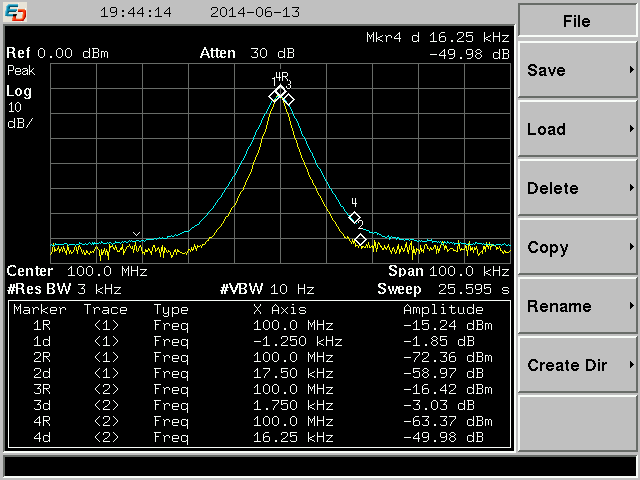
\includegraphics[width=8cm]
				{Imagenes/SCREN443.PNG}
				\caption{Espectros obtenidos con $RBW=300~Hz$ (en amarillo) y con $RBW=3~kHz$ (en celeste)}
				\label{Selec} 
		\end{figure}		
		
		%HUGO. Me encanta la THD 
		\subsubsection{Distorsi\'on arm\'onica de un generador de funciones}
		Cuando un sistema no lineal tiene una entrada que consiste en una se\~al senoidal de frecuencia $f_0$, a la salida de este sistema las frecuencia presentes son $f_0$ y m\'ultiplos de esta frecuencia $2f_0$,$3f_0$, etc, llamados arm\'onicos de la fundamental $f_0$.
		De esta manera se define la distorsi\'on arm\'onica cuyo valor da una idea de qu\'e tan lineal es el sistema y se define como
		$$THD=\frac{\sum_{n=1}^{+\infty}a^2_n}{a^2_0}$$
		Donde $a_n$ son los coeficientes de la serie de Fourier de cada componente de frecuencia $f_n$.
		En esta secci\'on se mide la THD del generador de funciones N9310A. Para ello se conecta el generador al analizador de espectros PSA 6000 por medio de un cable coaxil. La se\~nal del generador tiene una frecuencia de $500~MHz$. En la Figura \ref{THD} se puede observar las componentes espectrales de la se\~nal.
		\begin{figure}[!htb]
				\centering
				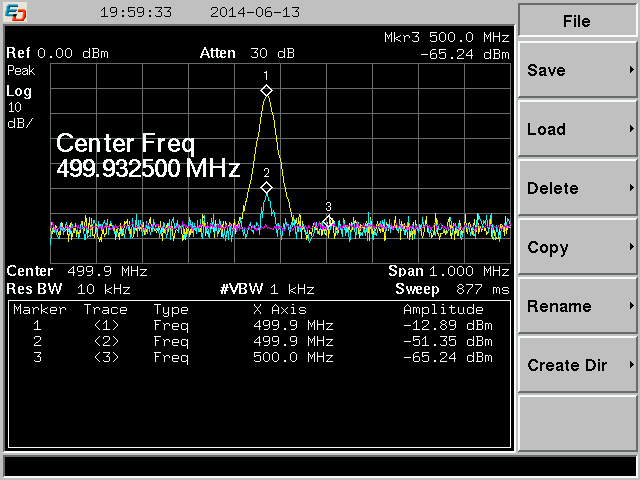
\includegraphics[width=8cm]
				{Imagenes/SCREN445.PNG}
				\caption{Frecuencia fundamental y primeros dos arm\'onicos de la se\~nal generada por el N9310A.}
				\label{THD} 
		\end{figure}
		Con lo cual puede calcularse la distrosi\'on, despreciando los arm\'onicos superiores al segundo
		$$THD=\frac{a^2_1+a^2_2}{a^2_0}$$
		$$THD=\frac{10^{\frac{-51.35}{5}}+10^{\frac{-65.24}{5}}}{10^{\frac{-12.89}{5}}}=10^{-7}$$
		%'No se si poner aca incerteza, creo que es m�s importante lo de abajo que es lo que espeficica el manual'. La verdad: Paja jajaja
		La cual es una distorsi\'on bastante baja. Por otra parte, el fabricante del generador asegura que las amplitudes de los arm\'onicos se encuentran $30~dB$ por debajo de la amplitud de la fundamental. Esto es f\'acil de comprobar ya que $A_0-A_1=(-12.89~dB\pm~1.5~dB)-(-51.35~dB\pm~1.5~dB)=38.46~dB~\pm~3~dB$, en cuyo peor ($35.46~~\pm~dB$) caso es mayor a lo especificado.
		%No esntendi mucho lo de la distorsi�n por. FRAN?			
		\subsubsection{Distorsi\'on por intermodulaci\'on del analizador de espectro}
		
		\subsubsection{Frecuencia de conversi\'on de un generador digital}
		Un generador de funciones digital, mediante un conversor digital-anal\'ogico, transforma una palabra de bits en un valor de tensi\'on. Evidentemente esta conversi\'on la realiza a determinada frecuencia ($125~MSa/s$), con lo cual es razonable que \'esta componente est\'e presente en el espectro de la se\~nal de salida del generador. En esta secci\'on, se busca obtener la frecuencia de convers\'on, $125~MHz$ y su amplitud respecto de la frecuencia de salida. En la Figura \ref{freqres} se puede ver la presencia de una componente residual que est\'a $88.5~dB~\pm~1.5~dB$ por debajo de la amplitud de la se\~nal de entrada que es de $0~dB~\pm~1.5~dB$. Como se esperaba su frecuencia es de $125~MHz~\pm~?~MHz$
		\begin{figure}[!htb]
				\centering
				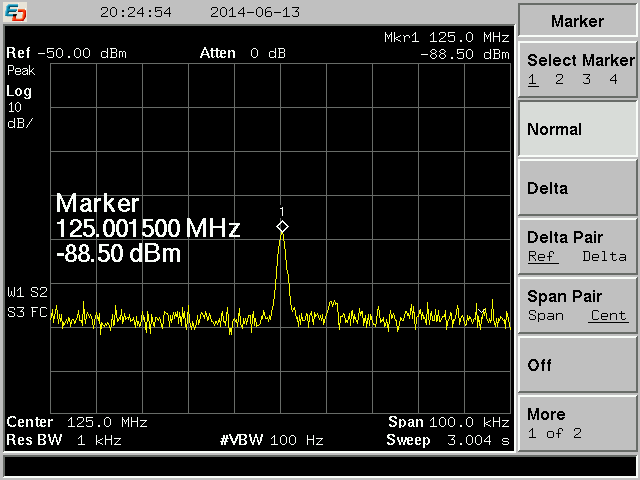
\includegraphics[width=8cm]
				{Imagenes/SCREN448.PNG}
				\caption{Espectro residual de la frecuencia del conversor digital-anal\'ogico del generador de se\~nales.}
				\label{freqres} 
		\end{figure}
		
		%HUGO. Preguntar phase noise
		\subsubsection{Ruido de fase}
		La especificaci\'on dada por el fabricante para el ruido de fase es 
		$$Phase Noise<-90~dBc/Hz$$
		
		\begin{figure}[!htb]
				\centering
				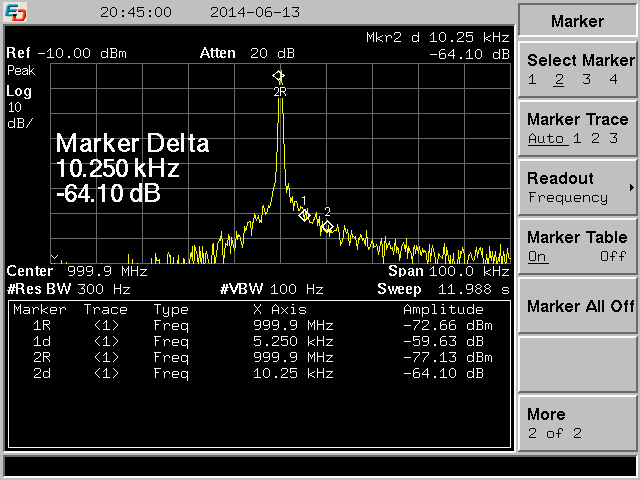
\includegraphics[width=8cm]
				{Imagenes/SCREN451.PNG}
				\caption{Medici\'on de ruido de fase.}
				\label{ruidofase} 
		\end{figure}
		
		\subsubsection{Modulaci\'on AM}
		En una modulaci\'on AM, la se\~nal que contiene la informaci\'on que se desea transmitir se utiliza para modular la amplitud de una se\~nal senoidal de frecuencia determinada, llamada portadora.
		Matem\'aticamente, si la se\~nal que se desea transmitir tiene un espectro $X(\omega)$, el espectro de la se\~nal modulada es $\Phi(\omega)=\frac{1}{2}X(\omega-\omega_c)+\frac{1}{2}X(\omega+\omega_c)+A\cdot\pi\cdot\delta(\omega-\omega_c)+A\cdot\pi\cdot\delta(\omega+\omega_c)$, donde $\omega_c$ es la frecuencia de la portadora y $A$ es una constante de la modulaci\'on. (Cuando la modulaci\'on no incluye las deltas en el espectro, se llama modulaci\'on AM con portadora suprimida)
		De todas maneras lo que se puede observar con el analizador de espectro es la parte correspondiente a las frecuencias positivas, es decir,
		$$\Phi(\omega)=\frac{1}{2}X(\omega-\omega_c)+A\cdot\pi\cdot\delta(\omega-\omega_c)$$
		Si la se\~nal a transmitir es senoidal de frecuencia angular $\omega_0$ y amplitud $f$, entonces el espectro que puede observarse en el analizador de espectro debe ser $$\Phi(\omega)=\frac{1}{2}f\cdot\pi\cdot\delta(\omega-(\omega_c-\omega_0))+\frac{1}{2}f\cdot\pi\cdot\delta(\omega-(\omega_c+\omega_0))+A\cdot\pi\cdot\delta(\omega-\omega_c)$$
		Al la relaci\'on $m_{AM}=\frac{f}{A}$ se la denomina \'indice de modulaci\'on y debe ser menor a 1 si la detecci\'on se realiza por envolvente.
		En esta secci\'on se utiliza el analizador de espectro para ver c\'omo var\'ian las componentes de una modulaci\'on AM al variar el \'indice de modulaci\'on, $m_{AM}$. Para ello se conecta el generador Siglent SDG1050 para crear una se\~nal modulada AM ($w_c=10~MHz$ y $w_0=2~kHz$) al analizador de espectro PSA 6000. En las Figuras \ref{AM1},\ref{AM2}y\ref{AM3} se pueden observar los espectros obtenidos para modulaciones con $m_{AM}=1$, $m_{AM}=0.25$ y $m_{AM}=0.03$, respectivamente. Las diferencias entre la amplitud de la portadora y las amplitudes laterales se pueden estimar a partir de la siguiente relaci\'on
		$$A_{diff}(dB)=20\cdot\log(\frac{2}{m_{AM}})$$
		En la Tabla\ref{AM}, se resumen los resultados obtenidos y se compara con el calculo te\'orico. Como se puede observar los resultados son cercanos y la incertidumbre de la medici\'on incluye los valores anal\'iticos.
		
		\begin{table}[!htp]
			\centering
			\begin{tabular}{|c|c|c|}
				\hline
				$m_{AM}$ & $A_{diff}(dB)$ (Medido) & $A_{diff}(dB)$(Estimado) \\
				\hline
				$1$ & $6.29~dB\pm~1.5~dB$& $6.02~dB$ \\
				\hline
				$0.25$ & $18.5~dB\pm~1.5~dB$& $18.06~dB$ \\
				\hline
				$0.03$ & $36~dB\pm~1.5~dB$& $36.47~dB$ \\															 	  	  
			\end{tabular}
			\caption{Diferencias entre las amplitudes de la portadora y la se\~nal de entrada obtenidas y estimadas} \label{AM}
		\end{table}	
		
		
		%HUGO. Las funciones de Bessel de FM son para mi jeje

		\begin{figure}[!htb]
				\centering
				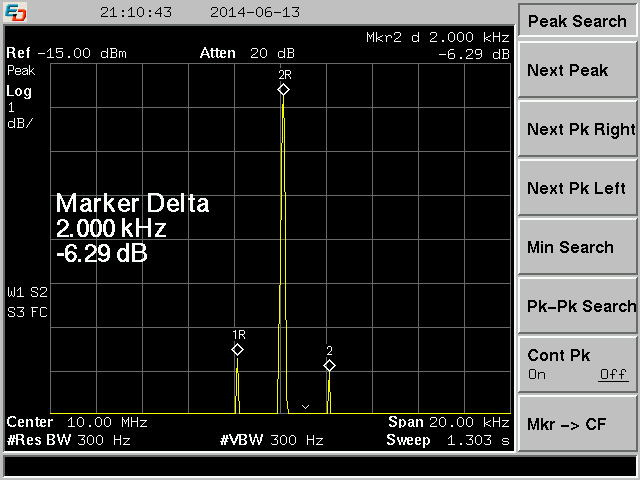
\includegraphics[width=8cm]
				{Imagenes/SCREN456.PNG}
				\caption{Espectro residual de la frecuencia del conversor digital-anal\'ogico del generador de se\~nales.}
				\label{AM1} 
		\end{figure}
		\begin{figure}[!htb]
				\centering
				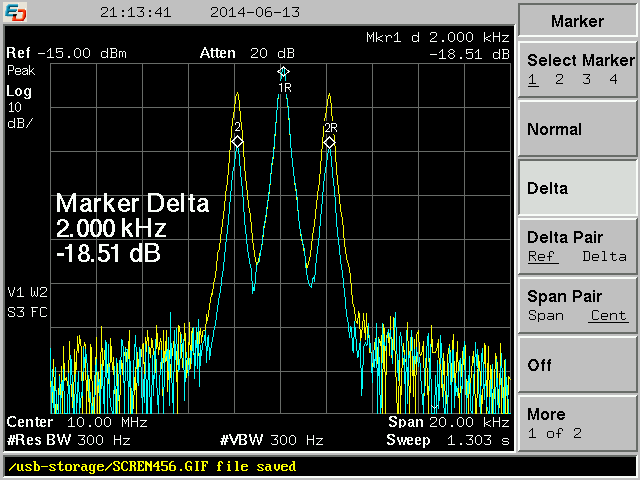
\includegraphics[width=8cm]
				{Imagenes/SCREN457.PNG}
				\caption{Espectro residual de la frecuencia del conversor digital-anal\'ogico del generador de se\~nales.}
				\label{AM2} 
		\end{figure}
		\begin{figure}[!htb]
				\centering
				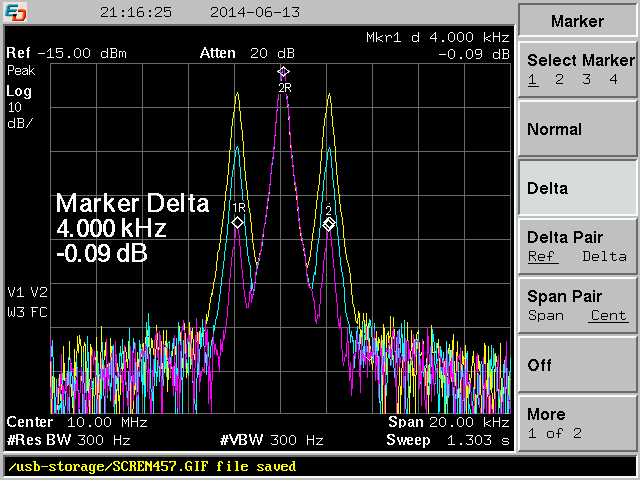
\includegraphics[width=8cm]
				{Imagenes/SCREN458.PNG}
				\caption{Espectro residual de la frecuencia del conversor digital-anal\'ogico del generador de se\~nales.}
				\label{AM3} 
		\end{figure}
		Por \'ultimo debe notarse que exiten diferencias entre las amplitudes de los picos laterales, cuando en teor\'ia deber\'ian ser id\'enticos. Las diferencias encontradas son de $0.4~dB$, $0.35~dB$ y $0.15~dB$ para $m_{AM}=1$, $m_{AM}=0.25$ y $m_{AM}=0.03$, respectivamente. Pero la incerteza de cada medici\'on es $\pm1.5~dB$ con lo cual no es posible conocer el origen de esta diferencia.
		\subsubsection{Modulaci\'on FM}
		Una modulaci\'on FM consiste b\'asicamente de modular la frecuencia de una se\~nal portadora con la se\~nal que contiene la informaci\'on que se desea transmitir. 
		Se puede demostrar que en una modulaci\'on FM, si la entrada a modular es del tipo $f_{in}=a\cdot \cos(w_{in}\cdot t)$, la se\~nal modulada es 
		$$\phi(t)=A\cdot\sum_{n=-\infty}^{+\infty}J_n(m_f)\cos((w_c+n\cdot w_{in})\cdot t)$$
		Donde $J_n(\cdot)$ es la funci\'on de Bessel de orden $n$ y $m_f$ es el \'indice de modulaci\'on. En la Figura \ref{bessel} se puede observar los gr\'aficos de la funci\'on de Bessel hasta el orden 5.
		\begin{figure}[!htb]
				\centering
				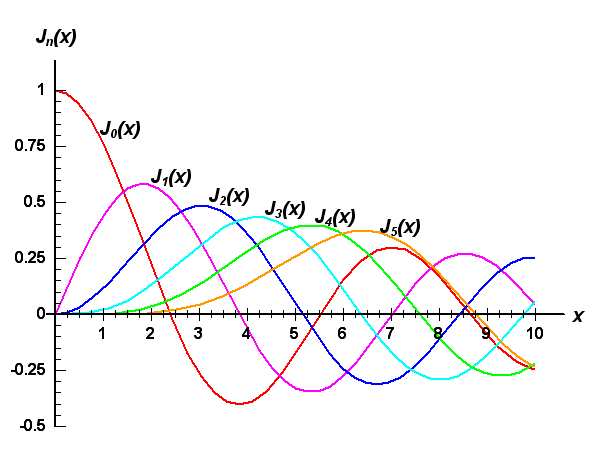
\includegraphics[width=8cm]
				{Imagenes/bessel.PNG}
				\caption{Funciones de Bessel.}
				\label{bessel} 
		\end{figure}\\
		Es decir que el espectro de salida ideal consiste en deltas ubicadas en $f=f_c,f_c\pm f_{in},f_c\pm 2f_{in},...$, cuyo pesao est\'a dado por $J_0(m_f),J_1(m_f),J_2(m_f),...$ respectivamente.
		Se propone encontrar los primeros dos ceros de la funci\'on de Bessel de orden 0. Esto se puede conseguir conectando un generador de modulaci\'on FM (Siglent SDG1050) al analizador de espectro PSA 6000 y modificando el \'indice de modulaci\'on hasta que la frecuencia portadora desaparezca (es decir, que $J_0(m_f)=0$).
		El primer cero se consigue cuando $f_{\mbox{desv\'io}}=4.8~kHz$, es decir cuando $m_f=\frac{f_{\mbox{desv\'io}}}{f_{\mbox{modulaci\'on}}}=\frac{4.8~kHz}{2~kHz}=2.4$. El cual es un valor bastante exacto, ya que matem\'aticamente el primer cero se encuentra en $z_1=2.4048$
		El segundo cero se encuentra cuando $f_{\mbox{desv\'io}}11.04~kHz$, es decir cuando $m_f==\frac{11.04~kHz}{2~kHz}=5.52$. Tambi\'en en este caso, el resultado obtenido es muy cercano al real, el cual es de $z_2=5.5201$
		Por otra parte en esta secci\'on se busca comprobar la ley emp\'irica de Carson, la cual postula que el $98\%$ de la potencia de una se\~nal est\'a comprendida dentro de un ancho de banda de
		$$BW=2\cdot(f_{\mbox{desv\'io}}+f_{\mbox{modulaci\'on}})$$.
		
		En las Figuras \ref{FM48}, \ref{FM10} y \ref{FM18}, se pueden ver los espectros obtenidos para modulaciones FM con $f_{\mbox{desv\'io}}=4.8~kHz$, $f_{\mbox{desv\'io}}=10~kHz$ y $f_{\mbox{desv\'io}}=18~kHz$, respectivamente. El analizador de espectro posee una funcionalidad que permite setear un porcentaje de potencia de la se\~nal modulada y devuelve el ancho de banda asociado a esa potencia.
		
		En la Tabla \ref{carson}, se pueden observar los resultados obtenidos utilizando el analizador de espetro para obtener el ancho de banda que contiene el $95\%$ de la potencia y el que se obtiene usando la regla de Carson.
			
		
		\begin{figure}[!htb]
				\centering
				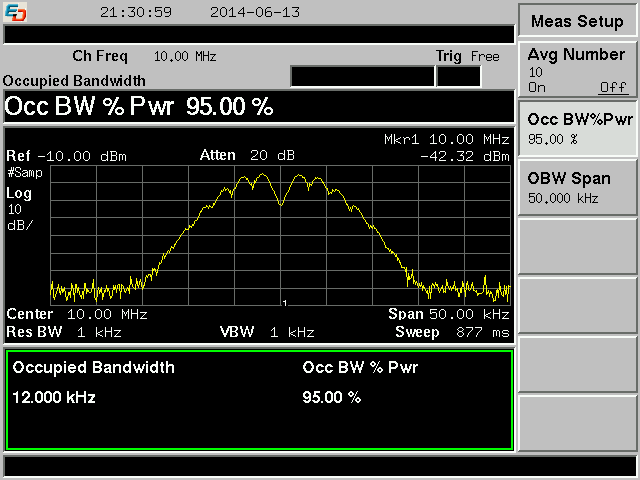
\includegraphics[width=8cm]
				{Imagenes/SCREN460.PNG}
				\caption{Espectro de una modulaci\'on FM, con $f_{\mbox{modulaci\'on}}=2~kHz$ y $f_{\mbox{desv\'io}}=4.8~kHz$.}
				\label{FM48} 
		\end{figure}		
		
		\begin{figure}[!htb]
				\centering
				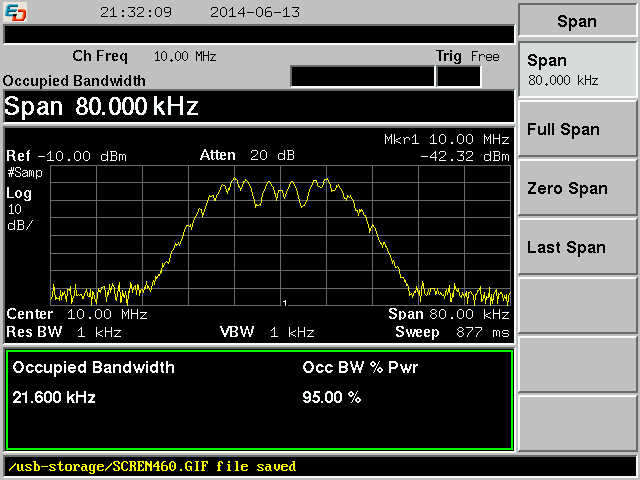
\includegraphics[width=8cm]
				{Imagenes/SCREN461.PNG}
				\caption{Espectro de una modulaci\'on FM, con $f_{\mbox{modulaci\'on}}=2~kHz$ y $f_{\mbox{desv\'io}}=10~kHz$.}
				\label{FM10} 
		\end{figure}		
		
		\begin{figure}[!htb]
				\centering
				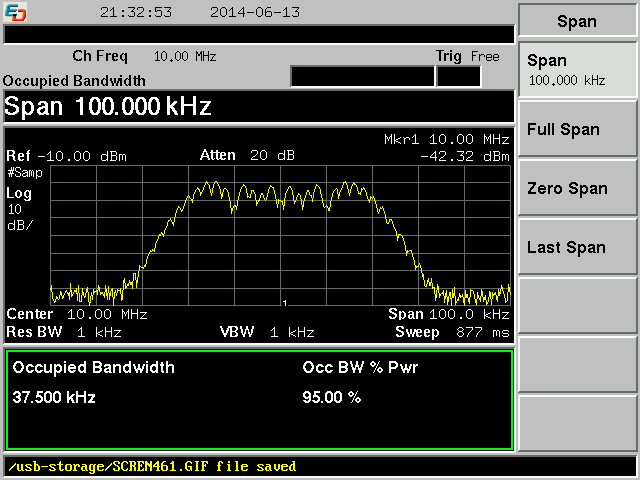
\includegraphics[width=8cm]
				{Imagenes/SCREN462.PNG}
				\caption{Espectro de una modulaci\'on FM, con $f_{\mbox{modulaci\'on}}=2~kHz$ y $f_{\mbox{desv\'io}}=18~kHz$.}
				\label{FM18} 
		\end{figure}
				\begin{table}[!htp]
					\centering
					\begin{tabular}{|c|c|c|c|}
						\hline
						$f_{\mbox{modulaci\'on}}$ & $f_{\mbox{desv\'io}}$ & $BW(Carson)$ & $BW(PSA 6000)$\\
						\hline
						$2~kHz$ & $4.8~kHz$& $13.6~kHz$ & $12~kHz$\\
						\hline
						$2~kHz$ & $10~kHz$& $24~kHz$ & $21.6~kHz$\\
						\hline
						$2~kHz$ & $18~kHz$& $40~kHz$ & $37.5~kHz$\\
						\hline						
						\hline
					\end{tabular}
					\caption{Resultados obtenidos para calcular el ancho de banda de potencia} \label{carson}
				\end{table}	
		Como era  esperado, de la Tabla puede notarse  que el ancho de banda obtenido usando la regla de Carson es pr\'oximo al obtenido con el analizador de espectro. Por otra parte, debe notarse que el ancho de banda obtenido usando la regla de Carson es mayor, lo cual es l\'ogico pues la potencia de la se\~nal que abarca ($98\%$) es mayor que el que se calcula con el analizador de espectro ($95\%$).
		\subsubsection{Figura de ruido}
		La figura de ruido de un dispositivo se define como la degradaci\'on de la relaci\'on se\~nal a ruido, que sufre una se\~nal cuando para a trav\'es de un dispositivo. Matem\'aticamente puede expresarse como $$F=\frac{\frac{S_i}{N_i}}{\frac{S_o}{N_o}}$$
		Para el analizador de espectro, \'esta expresi\'on puede simplificarse ya que la ganancia del analizador es unitaria con lo cual $\frac{S_o}{S_i}=1$ entonces
		$$F=\frac{N_o}{N_i}$$
		Colocando a la entrada del analizador de espectro una carga de $50\Omega$, el ruido a la entrada se convierte en 
		$$N_i(dB)=kTB=-174~dBm$$, donde $k$ es la constante de Boltzmann, $T$ es la temperatura absoluta en Kelvin y $B$ es el ancho de banda seleccionado.
		En la Figura \ref{noise}, se muestra el resultado obtenido de medir el ruido de salida. Con la entrada adaptada a $50\Omega$ se puede ir variando la secci\'on del espectro a considerar para obtener su densidad espectral de potencia. Como se puede ver se obtiene $N_o(dB)=kTB=-145.52~dBm$ con lo cual
		$$F(dB)=N_o(dB)-N_i(dB)=-145.52~dBm-(-174~dBm)=28.48~dB$$
		\begin{figure}[!htb]
				\centering
				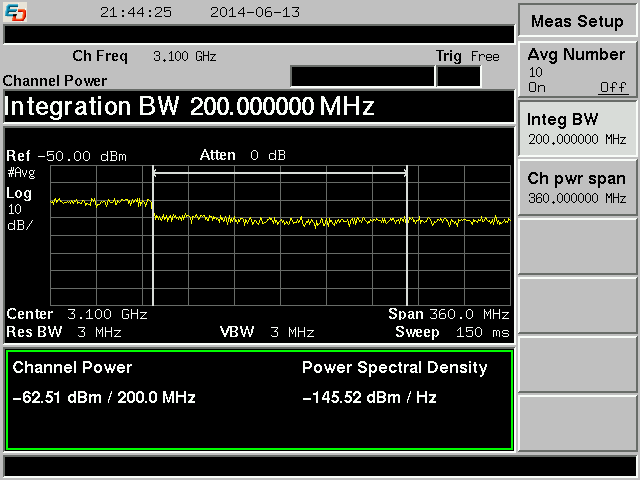
\includegraphics[width=8cm]
				{Imagenes/SCREN464.PNG}
				\caption{Ruido a la salida  analizador de espectro.}
				\label{noise} 
		\end{figure}
		Es importante notar que esta figura de ruido tambi\'en depende de la banda de frecuencias en la que se calcule la potencia de ruido de salida. De hecho Agilent tiene especificado el nivel de ruido para 3 rangos de frecuencia.
		\begin{itemize}
			\item $N_o(dB)\leq-105~dBm$: 	$150~kHz-1~GHz$
			\item $N_o(dB)\leq-100~dBm$:	 $1~GHz-2.4~GHz$
			\item $N_o(dB)\leq-95~dBm$:	 $2.4~GHz-6.2~GHz$
		\end{itemize}
		Las cuales pueden traducirse en especificaciones de figura de ruido, $F$, restando la potencia de ruido de entrada
		\begin{itemize}
			\item $F\leq69-~dB$: 	$150~kHz-1~GHz$
			\item $F\leq74~dB$:	 $1~GHz-2.4~GHz$
			\item $F\leq79~dB$:	 $2.4~GHz-6.2~GHz$
		\end{itemize}
		Dado que se opera en una regi\'on centrada en $3~GHz$, la especificaci\'on se corresponde con la tercer banda ($2.4~GHz-6.2~GHz$) y c\'omo se puede advertir se cumple holgadamente, $28.48~dB\ll79~dB$.
		
	\subsection{Mediciones con el analizador de redes}
		\subsubsection{Transferencia de un pasabanda}
		En esta secci\'on se busca obtener, utilizando el analizador de redes, la funci\'on de trasferencia de un pasabanda PolyPhaser  cuya banda de paso se especifica en  $800~MHz-900~MHz$. En la Figura \ref{transferenciabandpass} se observa la tranferencia obtenida al medir con el analizador Agilent N9923A. Como se puede observar el ancho de banda obtenido es mayor al especificado por el fabricante, probablemente esto se deba al bajo nivel de potencia con el cual se est\'a realizando la medici\'on, ya que la especificaci\'on est\'a referida a un nivel de potencia de $750~W$
		
		%CAMBIAR IMAGENNNNNNNNNNNNNNNNNNNNN
		\begin{figure}[!htb]
				\centering
				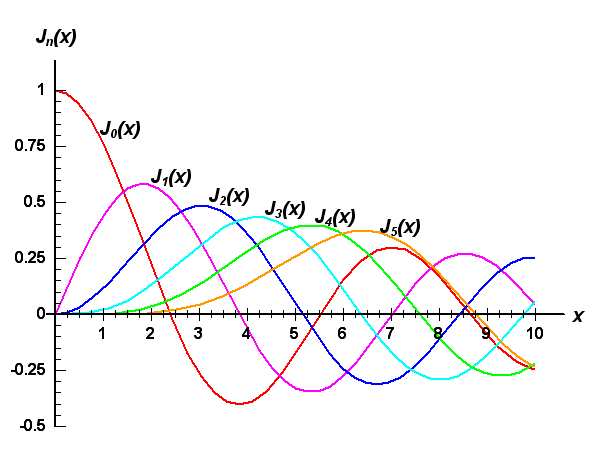
\includegraphics[width=8cm]
				{Imagenes/bessel.PNG}
				\caption{Tranferencia (par\'ametro $S_{21}$) del pasabanda.}
				\label{transferenciabandpass} 
		\end{figure}
		\subsubsection{Transferencia de 2 cables coaxiles}
		En esta secc\'on se  busca obtener la transferencia de dos cables coaxiles de $Z_0=50~\Omega$, uno fino y otro grueso. En ambos casos para se deb\'io recurrir a la utilizaci\'on conectores extra para poder conectar los coaxiles con el analizador de redes, por lo tanto en su transferencia se incluye tambi\'en el efecto de estos conectores. En las Figuras \ref{caoxilflaco} y \ref{coaxilgordo}, se muestran las transferencias obtenidas para el cable coaxil fino y el grueso, respectivamente.
		%CAMBIAR IMAGENNNNNNNNNNNNNNNNNNNNN
		\begin{figure}[!htb]
				\centering
				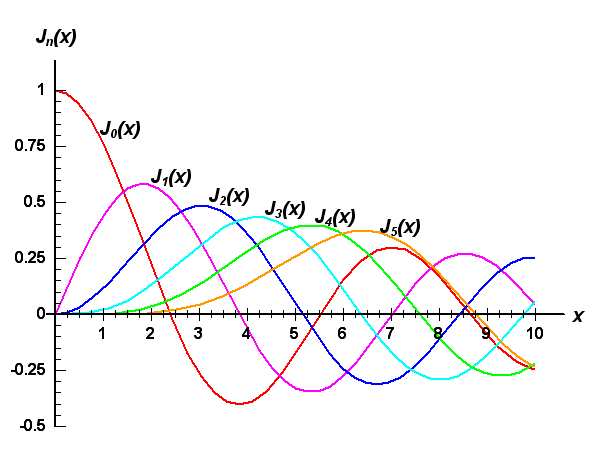
\includegraphics[width=8cm]
				{Imagenes/bessel.PNG}
				\caption{Tranferencia (par\'ametro $S_{21}$)del cable coaxil fino.}
				\label{caoxilflaco} 
		\end{figure}
		%CAMBIAR IMAGENNNNNNNNNNNNNNNNNNNNN
		\begin{figure}[!htb]
				\centering
				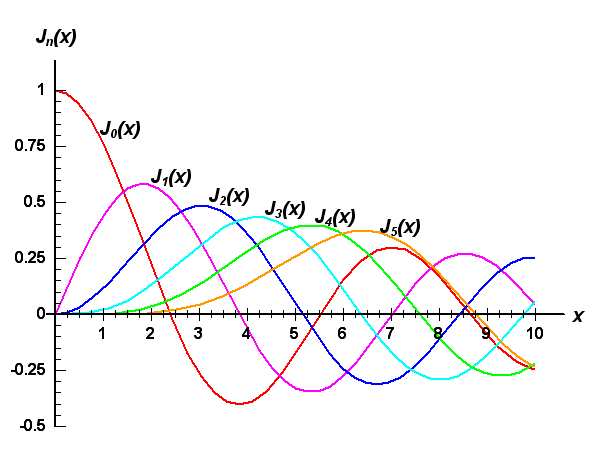
\includegraphics[width=8cm]
				{Imagenes/bessel.PNG}
				\caption{Tranferencia (par\'ametro $S_{21}$) del cable coaxil grueso.}
				\label{coaxilgordo} 
		\end{figure}
		Para poder analizar el efecto de los conectores se quita el cable coaxil, y se dejan a \'estos conectados al analizador para poder obtener su transferencia, la cual se grafica en la Figura \ref{tranferenciaconectorrr}
		%CAMBIAR IMAGENNNNNNNNNNNNNNNNNNNNN
		\begin{figure}[!htb]
				\centering
				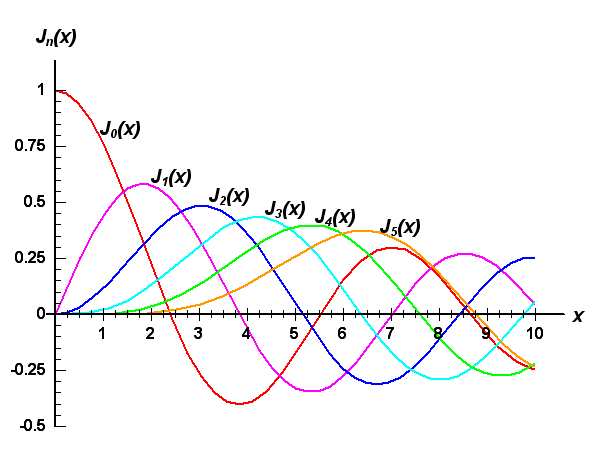
\includegraphics[width=8cm]
				{Imagenes/bessel.PNG}
				\caption{Tranferencia (par\'ametro $S_{21}$) de los conectores.}
				\label{tranferenciaconectorrr} 
		\end{figure}
		\subsubsection{Impedancia de entrada}
		En esta secci\'on la medici\'on a realizar es la de obtener las impedancias de entrada de alguno de los instrumentos que han sido utilizados en el laboratorio. La forma m\'as conveniente de presentar el resultado es utilizando la carta de Smith, ya que muestra como var\'ia a impedancia, en su parte real e  imaginaria, a medida que var\'ia la frecuencia.
		\begin{itemize}
			\item Analizador de espectro HM 5006
		\end{itemize}
		En la Figura \ref*{tranferenciacHM}, se puede ver que para la frecuencia de corte especificada por el fabricante, $500~MHz$, la impedancia de entrada es de $4564564$, la cual se corresponde con la especificada de $50~\Omega$.
		%CAMBIAR IMAGENNNNNNNNNNNNNNNNNNNNN
		\begin{figure}[!htb]
				\centering
				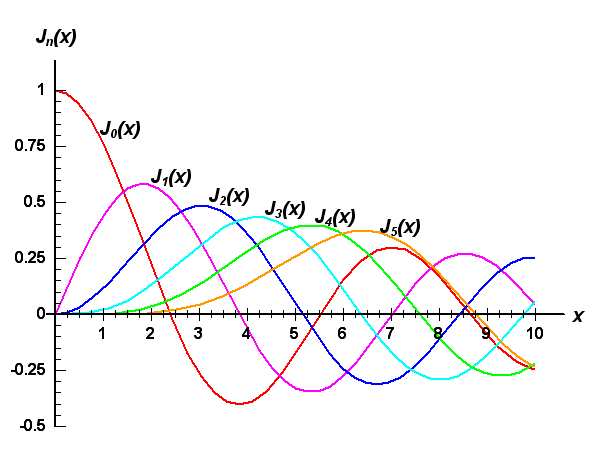
\includegraphics[width=8cm]
				{Imagenes/bessel.PNG}
				\caption{Carta de Smith de la impedancia del analizador HM 5006.}
				\label{tranferenciacHM} 
		\end{figure}		
		\begin{itemize}
			\item Impedanc\'imetro HP 4815A
		\end{itemize}
		El impedanc\'imetro opera hasta una frecuencia de $108~MHz$, con lo cual es deseable que su impedancia de entrada se comporte de manera constante en ese rango. En la Figura \ref*{tranferenciaimpedanciamiterro} se puede observar el resultado obtenido.
		%CAMBIAR IMAGENNNNNNNNNNNNNNNNNNNNN
		\begin{figure}[!htb]
				\centering
				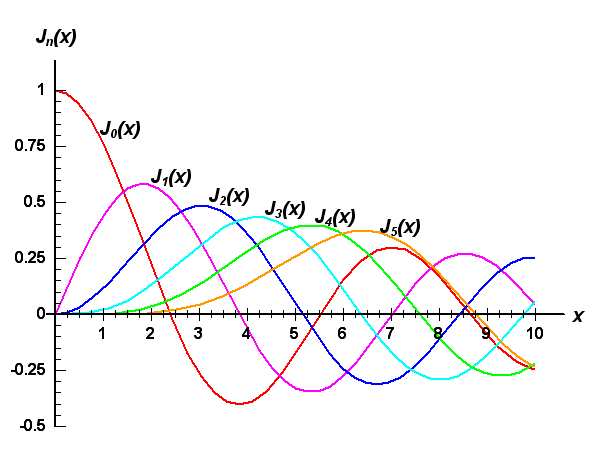
\includegraphics[width=8cm]
				{Imagenes/bessel.PNG}
				\caption{Carta de Smith de la impedancia del impedanc\'imetro HP 4815A}
				\label{tranferenciaimpedanciamiterro} 
		\end{figure}		
	\section{Conclusiones}
	\indent
\end{document}